\section{Experiments}
\label{sec:experiments}
\vspace{-2mm}

\subsection{Experimental setups}
\vspace{-1mm}

To validate the generality of \implname we consider three pre-trained LLMs ranging across different model families and architecture sizes: \llama, \mistral, and \llamaXL. 
For each model, we obtain three sets of $z$ vectors to maximize performance for GSM8K~\citep{cobbe2021training},  MBPP-pro~\citep{austin2021program}, and ARC-Easy~\citep{clark2018think}, respectively.
Additionally, we train a set of $z$ vectors for \llama, when applied as the language backbone for TextVQA~\citep{singh2019towards}.
Finally, we evaluate the \implname on four unseen tasks: MATH~\citep{hendrycks2021measuring}, Humaneval~\citep{chen2021evaluating}, ARC-Challenge~\citep{clark2018think}, and OKVQA~\citep{marino2019ok}. 
In our adaptation experiments, we only consider experts obtained in the pure-language settings.
Please refer to Appendix~\ref{app:sec:implementation} for additional details and hyper-parameters summary.

\vspace{-2mm}
\subsection{Experimental results}

% \begin{table}[!t]
% \centering

% \caption{\textbf{LLM Fine-tuning Results.} LLM performance on the test splits.}

% \small
% \begin{tabular}{llll}
% \toprule

% \textbf{Method} & \textbf{GSM8K} & \textbf{MBPP-Pro} & \textbf{ARC-Easy} \\

% \midrule
% \llama & {\normalsize 75.89 {\footnotesize (\grey{1.00})}} & {\normalsize 64.65 {\footnotesize (\grey{1.00})}} & {\normalsize 88.59 {\footnotesize (\grey{1.00})}} \\
% \quad + LoRA & {\normalsize 70.58 {\footnotesize (\red{0.93})}} & \textbf{{\normalsize 67.68 {\footnotesize (\green{1.05})}}} & {\normalsize 88.97 {\footnotesize (\grey{1.00})}} \\
% \quad + SVF (Ours) & \textbf{{\normalsize 79.15 {\footnotesize (\green{1.04})}}} & {\normalsize 66.67 {\footnotesize (\green{1.03})}} & \textbf{{\normalsize 89.56 {\footnotesize (\green{1.01})}}} \\

% \midrule
% \mistral & {\normalsize 42.83 {\footnotesize (\grey{1.00})}} & {\normalsize 49.50 {\footnotesize (\grey{1.00})}} & {\normalsize 49.50 {\footnotesize (\grey{1.00})}} \\
% \quad + LoRA & {\normalsize 36.09 {\footnotesize (\red{0.84})}} & {\normalsize 47.47 {\footnotesize (\red{0.96})}} & {\normalsize 47.47 {\footnotesize (\red{0.96})}} \\
% \quad + SVF (Ours) & \textbf{{\normalsize 49.74 {\footnotesize (\green{1.16})}}} & \textbf{{\normalsize 51.52 {\footnotesize (\green{1.04})}}} & \textbf{{\normalsize 85.14 {\footnotesize (\green{1.72})}}} \\

% \midrule
% \llamaXL & {\normalsize 85.29 {\footnotesize (\grey{1.00})}} & \textbf{{\normalsize 80.81 {\footnotesize (\grey{1.00})}}} & \textbf{{\normalsize 89.10 {\footnotesize (\grey{1.00})}}} \\
% \quad + SVF (Ours) & \textbf{{\normalsize 88.32 {\footnotesize (\green{1.04})}}} & \textbf{{\normalsize 80.81 {\footnotesize (\grey{1.00})}}} & {\normalsize 88.47 {\footnotesize (\red{0.99})}} \\

% \bottomrule
% \end{tabular}

% \label{tab:res:svf_train_tasks}
% \end{table}

% \begin{figure}[!t]
%     \centering
%     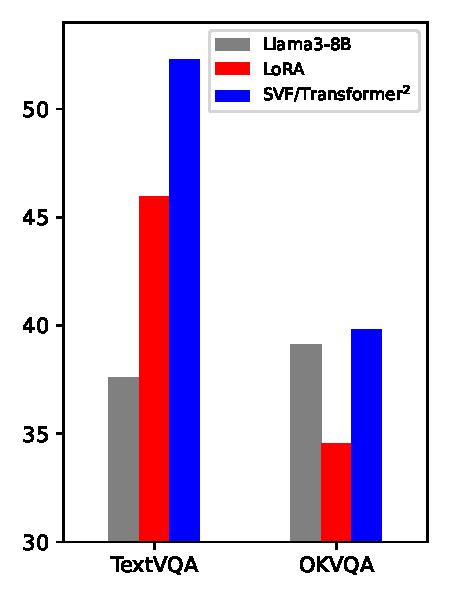
\includegraphics[width=\textwidth]{images/vlm_barplot.pdf}
%     % \vspace{-8mm}
%     \caption{\textbf{VLM Results.}
%     }
%     % \vspace{-4mm}
%     \label{fig:vlm_results}
% \end{figure}



\begin{figure}[!b]
    \vspace{-4mm}
    \centering

    % Left side: Table
    \begin{minipage}{0.75\linewidth}
        \centering
        \captionof{table}{\textbf{Fine-tuning results.} LLM performance on the test splits of math, coding and reasoning. Normalized scores are in the parentheses.}
        \vspace{-3.5mm}
        \small
        \begin{tabular}{llll}
            \toprule
            \textbf{Method} & \textbf{GSM8K} & \textbf{MBPP-Pro} & \textbf{ARC-Easy} \\
            \midrule
            \llama & {\normalsize 75.89 {\scriptsize (\grey{1.00})}} & {\normalsize 64.65 {\scriptsize (\grey{1.00})}} & {\normalsize 88.59 {\scriptsize (\grey{1.00})}} \\
            \quad + LoRA & {\normalsize 77.18 {\scriptsize (\green{1.02})}} & \textbf{{\normalsize 67.68 {\scriptsize (\green{1.05})}}} & {\normalsize 88.97 {\scriptsize (\grey{1.00})}} \\
            \quad + SVF (Ours) & \textbf{{\normalsize 79.15 {\scriptsize (\green{1.04})}}} & {\normalsize 66.67 {\scriptsize (\green{1.03})}} & \textbf{{\normalsize 89.56 {\scriptsize (\green{1.01})}}} \\
            \midrule
            \mistral & {\normalsize 42.83 {\scriptsize (\grey{1.00})}} & {\normalsize 49.50 {\scriptsize (\grey{1.00})}} & {\normalsize 81.65 {\scriptsize (\grey{1.00})}} \\
            \quad + LoRA & {\normalsize 44.66 {\scriptsize (\red{1.04})}} & {\normalsize 51.52 {\scriptsize (\green{1.04})}} & {\normalsize 81.19 {\scriptsize (\red{0.98})}} \\
            \quad + SVF (Ours) & \textbf{{\normalsize 49.74 {\scriptsize (\green{1.16})}}} & \textbf{{\normalsize 51.52 {\scriptsize (\green{1.04})}}} & \textbf{{\normalsize 85.14 {\scriptsize (\green{1.04})}}} \\
            \midrule            
            \llamaXL & {\normalsize 85.29 {\footnotesize (\grey{1.00})}} & \textbf{{\normalsize 80.81 {\footnotesize (\grey{1.00})}}} & \textbf{{\normalsize 89.10 {\footnotesize (\grey{1.00})}}} \\
            \quad + LoRA & {\normalsize 77.26 {\footnotesize (\red{0.91})}} & {\normalsize 68.69 {\footnotesize (\red{0.85})}} & {\normalsize 88.55 {\footnotesize (\red{0.99})}} \\
            \quad + SVF (Ours) & \textbf{{\normalsize 88.32 {\footnotesize (\green{1.04})}}} & \textbf{{\normalsize 80.81 {\footnotesize (\grey{1.00})}}} & {\normalsize 88.47 {\footnotesize (\red{0.99})}} \\
            \bottomrule                
        \end{tabular}
        \label{tab:res:svf_train_tasks}
    \end{minipage}
    \hfill
    % Right side: Figure
    \begin{minipage}{0.23\linewidth}
        \centering
        % \vspace{2mm}
        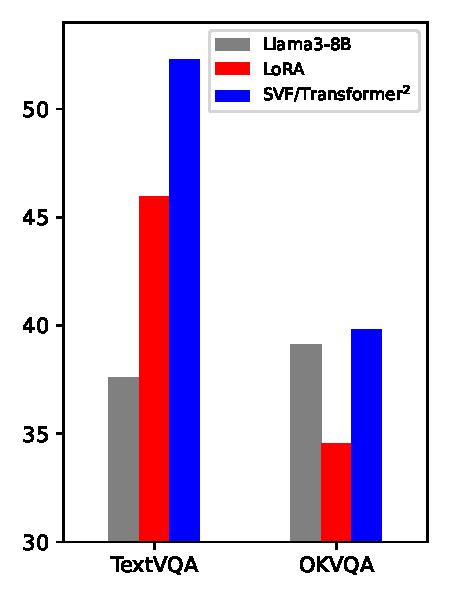
\includegraphics[width=\linewidth]{images/vlm_barplot.pdf}
        \vspace{-8mm}
        \captionof{figure}{\textbf{Results for the VLM domain.}}
        \label{fig:vlm_results}
    \end{minipage}

\end{figure}



\textbf{\svdacro performance}
resources, with less than 10\% of the training parameters of our LoRA implementation.
We provide results training on each considered task with the \llama, \mistral, and \llamaXL base models in Table~\ref{tab:res:svf_train_tasks}.
Remarkably, we find that \svdacro provides considerable performance gains across nearly all tasks and base models. Instead, LoRA experts yield smaller gains and even sporadic performance degradation.
To ensure a fair comparison, we provide extensive ablations to both our model and the LoRA baseline considering different architecture and optimization objectives in Appendix~ \ref{app:sec:ablation_studies}).


\textbf{Adaptation performance}
With the \svdacro trained $z$ vectors, we assess the self-adaptation capability of \implname on unseen tasks.
As shown in Table~\ref{tab:res:svf_ada_tasks}, all of our \implname adaptation strategies demonstrate improvements across all tasks for nearly all the models.
In contrast, even the best training LoRAs only provide marginal improvements on the ARC-Challenge task and still significantly deteriorate performance on both MATH and Humaneval. 
Comparing the three proposed adaptation strategies, we highlight a clear monotonic trend -- with more involved strategies and additional information about the test-time condition, self-adaptation appears to be increasingly effective.
This trend shows that providing additional or different kinds of information seems to be highly beneficial to our framework, suggesting that \implname could provide foundation models with new means to continually improve performance when deployed in lifelong settings.

\begin{table}[!t]
\centering
\vspace{-2mm}
\caption{\textbf{Self-adaptation on unseen tasks.} Normalized scores are in the parentheses.}
% \vspace{-2mm}
\small
\begin{tabular}{llll}
\toprule
Method & MATH & Humaneval & ARC-Challenge \\

\midrule
\llama3 & {\normalsize 24.54 {\footnotesize (\grey{1.00})}} & {\normalsize 60.98 {\footnotesize (\grey{1.00})}} & {\normalsize 80.63 {\footnotesize (\grey{1.00})}} \\
\quad + LoRA & {\normalsize 21.68 {\footnotesize (\red{0.88})}} & {\normalsize 52.44 {\footnotesize (\red{0.86})}} & {\normalsize 81.06 {\footnotesize (\green{1.01})}} \\
\quad + \implname (Prompt) & {\normalsize 25.22 {\footnotesize (\green{1.03})}} & {\normalsize 61.59 {\footnotesize (\green{1.01})}} & {\normalsize 81.74 {\footnotesize (\green{1.01})}} \\
\quad + \implname (Cls-expert) & {\normalsize 25.18 {\footnotesize (\green{1.03})}} & {\normalsize 62.80 {\footnotesize (\green{1.03})}} & {\normalsize 81.37 {\footnotesize (\green{1.01})}} \\
\quad + \implname (Few-shot) & \textbf{{\normalsize 25.47 {\footnotesize (\green{1.04})}}} & \textbf{{\normalsize 62.99 {\footnotesize (\green{1.03})}}} & \textbf{{\normalsize 82.61 {\footnotesize (\green{1.02})}}} \\

\midrule
\mistral & {\normalsize 13.02 {\footnotesize (\grey{1.00})}} & {\normalsize 43.29 {\footnotesize (\grey{1.00})}} & {\normalsize 71.76 {\footnotesize (\grey{1.00})}} \\
\quad + LoRA & {\normalsize 11.18 {\footnotesize (\red{0.86})}} & {\normalsize 31.71 {\footnotesize (\red{0.73})}} & \textbf{{\normalsize 75.77 {\footnotesize (\green{1.06})}}} \\
\quad + \implname (Prompt) & {\normalsize 11.86 {\footnotesize (\red{0.91})}} & {\normalsize 43.90 {\footnotesize (\green{1.01})}} & {\normalsize 72.35 {\footnotesize (\green{1.01})}} \\
\quad + \implname (Cls-expert) & {\normalsize 11.60 {\footnotesize (\red{0.89})}} & {\normalsize 43.90 {\footnotesize (\green{1.01})}} & {\normalsize 74.83 {\footnotesize (\green{1.04})}} \\
\quad + \implname (Few-shot) & \textbf{{\normalsize 13.39 {\footnotesize (\green{1.03})}}} & \textbf{{\normalsize 47.40 {\footnotesize (\green{1.09})}}} & {\normalsize 75.47 {\footnotesize (\green{1.05})}} \\

\midrule
\llamaXL & \textbf{{\normalsize 40.64 {\footnotesize (\grey{1.00})}}} & {\normalsize 78.66 {\footnotesize (\grey{1.00})}} & {\normalsize 87.63 {\footnotesize (\grey{1.00})}} \\
\quad + LoRA & {\normalsize 25.40 {\footnotesize (\red{0.62})}} & {\normalsize 73.78 {\footnotesize (\red{0.94})}} & {\normalsize 83.70 {\footnotesize (\red{0.96})}} \\
\quad + \implname (Prompt) & {\normalsize 40.44 {\footnotesize (\grey{1.00})}} & \textbf{{\normalsize 79.88 {\footnotesize (\green{1.02})}}} & \textbf{{\normalsize 88.48 {\footnotesize (\green{1.01})}}} \\
\bottomrule

\end{tabular}

\label{tab:res:svf_ada_tasks}
\vspace{-6mm}
\end{table}



\vspace{-2mm}
\subsection{Cross-model analysis}
\vspace{-2mm}
\label{sec:analysis}
We explore the potential for our self-adaptation framework to be applied \textit{across different LLMs}. We evaluate whether the \svdacro expert vectors trained on \llama can benefit \mistral, and whether we can perform adaptation across the expert vectors of these two models. We present our main findings in Table~\ref{tab:analysis:cross_model_main} and refer to Appendix~\ref{app:sec:additional_exp} for additional detailed results. 
Surprisingly, positive transfer does occur across the two models, with visible benefits in 2 out of 3 tasks.
We note these improvements are due to the inherent ordering of the \svdacro parameterization, as \textit{randomly shuffling} each \svdacro vector before applying it to the Mistral model consistently degrades performance. 
This operation leads to notable performance degradation across tasks. 
Finally, by performing few-shot adaptation using the \svdacro vectors collected from both models, the performance of \mistral further improves across the board.
We observe that these gains even surpass the best score from adapting \mistral with \textit{all} the \svdacro vectors in the ARC-Challenge task reported in Table~\ref{tab:res:svf_ada_tasks}.  
While these results appear promising, we note that the surprising compatibility discovered through our naive transfer approach is potentially tied to the similarity between the architectures of the two considered LLMs.
To this end, whether similar transfer can be replicated with models of different scales remains an open research question that could open the doors to disentangling and recycling task-specific skills for models, with important implications for the democratization and sustainability of the field.

\vspace{-4mm}
\begin{table}[!h]
% \vspace{-4mm}
% \caption{\textbf{Cross-model $z$ vector transfer.}
\caption{\textbf{Cross-model $\boldsymbol{z}$ vector transfer.}
Results from transferring the expert vectors trained on \llama to \mistral with cross model few-shot adaptation.
}
% \vspace{-3.5mm}
\centering
\begin{tabular}{lccc}
\toprule
\textbf{Method} & \textbf{MATH} & \textbf{Humaneval} & \textbf{ARC-Challenge} \\
\textit{SVF training task} & \small{\textit{GSM8K}} & \small{\textit{MBPP-pro}} & \small{\textit{ARC-Easy}} \\
\midrule


\textsc{Mistral-7B-Instruct-v0.3} & \textbf{{\normalsize 13.02 {\footnotesize (\grey{1.00})}}} & {\normalsize 43.29 {\footnotesize (\grey{1.00})}} & {\normalsize 71.76 {\footnotesize (\grey{1.00})}} \\

\midrule

\quad + Llama SVF (ordered $\sigma_i$) & {\normalsize 11.96 {\footnotesize (\red{0.92})}} & {\normalsize 45.12 {\footnotesize (\green{1.04})}} & {\normalsize 72.01 {\footnotesize (\grey{1.00})}} \\
\quad + Llama SVF (shuffled $\sigma_i$) & {\normalsize 10.52 {\footnotesize (\red{0.81})}} & {\normalsize 40.24 {\footnotesize (\red{0.93})}} & {\normalsize 70.82 {\footnotesize (\red{0.99})}} \\
\quad + Few-shot adaptation (cross-model) & {\normalsize 12.65 {\footnotesize (\red{0.97})}} & \textbf{{\normalsize 46.75 {\footnotesize (\green{1.08})}}} & \textbf{{\normalsize 75.64 {\footnotesize (\green{1.05})}}} \\

\bottomrule
\end{tabular}
\label{tab:analysis:cross_model_main}
\vspace{-2mm}
\end{table}